\section{1174095 - Muhammad Dzihan Al-Banna}
    \subsection{Teori}
    \begin{enumerate}
        \item Kenapa file suara harus dilakukan MFCC
        \subitem digunakan untuk mengidentifikasi jenis suara misalkan jenis suara gendre lagu jes pop metal dan klasikal atau suara ultra sonic. 
        
        \begin{figure}[H]
            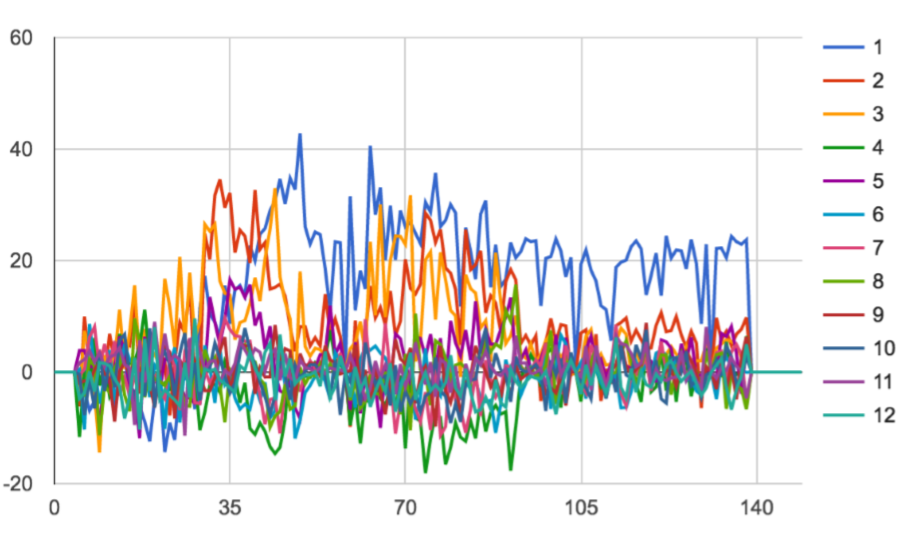
\includegraphics[width=4cm]{figures/1174095/tugas6/teori1.png}
            \centering
              \caption{Ilustrasi MFCC}
        \end{figure}
        
        \item Konsep dasar Neural Network
        \subitem konsep neural network dilaka ada inputan pasti ada outputan sesuai dengan kategori inputan dan fungsi di dalamnya.
        
        \begin{figure}[H]
            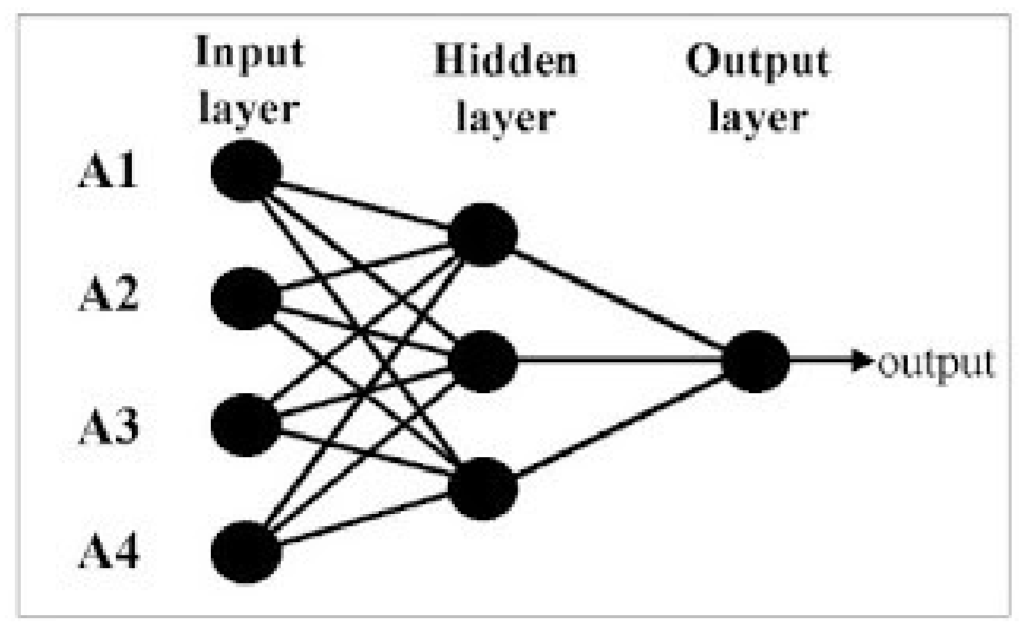
\includegraphics[width=4cm]{figures/1174095/tugas6/teori2.png}
            \centering
              \caption{Ilustrasi Neural Network}
        \end{figure}
        
        \item Konsep Pembobotan dalam Neural Network
        \subitem pembobotan dalam neural network yaitu digunakan untuk membedakan objek inputan atau variabel inputan untuk AI misalkan apel dan jeruk digunakan untuk variabel inputan maka dibuat pembobotan anatara kedua benda tersebut untuk menentukan output yang pasti dari inputan yang dilakukan
        
        \begin{figure}[H]
            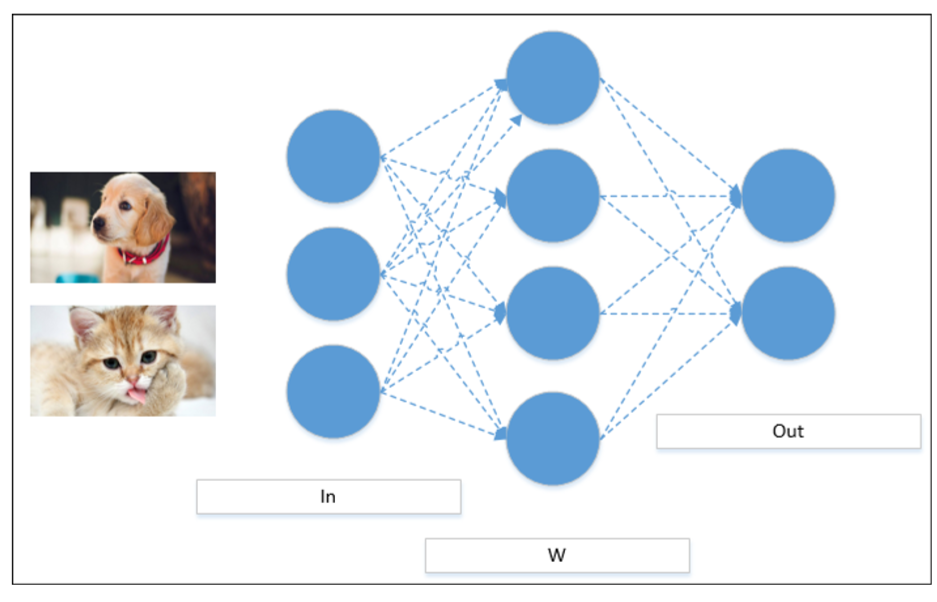
\includegraphics[width=4cm]{figures/1174095/tugas6/teori3.png}
            \centering
              \caption{Ilustrasi pembobotan Neural Network}
              
        \end{figure}
        
        \item Konsep Aktifasi dalam Neural Network
        \subitem cara aktifitas dalam neural network dilakukan terhadap input pada neural network inputan tersebut dimasukan kepada fungsi pada mesin misalkan fungsi tanh(x) sehingga di hasilkanlah output yang sesuai dengan fungsi tersebut.
        
        \begin{figure}[H]
            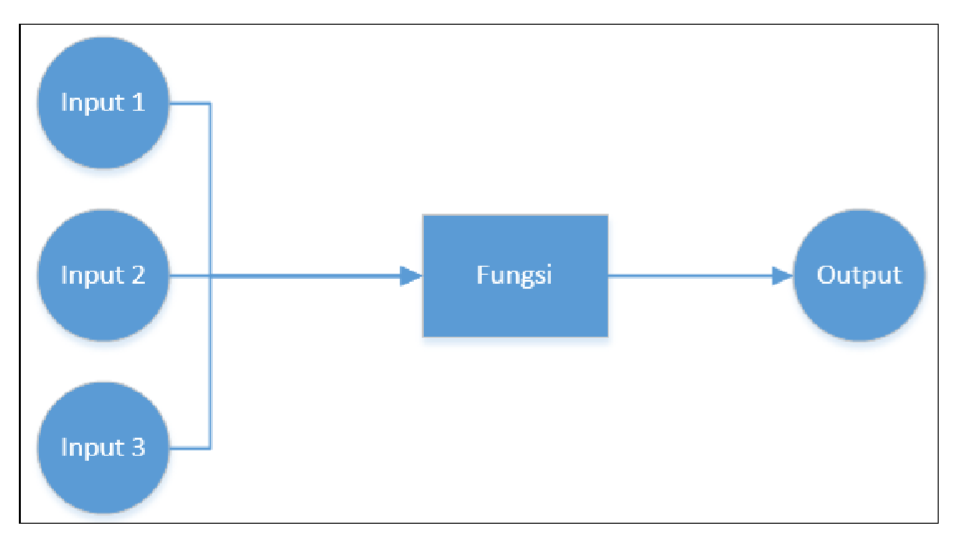
\includegraphics[width=4cm]{figures/1174095/tugas6/teori4.png}
            \centering
              \caption{Ilustrasi fungsi aktifasi Neural Network}
              \label{f4}
        \end{figure}
        
        \item cara membaca hasil PLOT dari MFCC
	\subitem cara membaca hasil ploting dari MFCC yaitu tentukan terlebih dahulu batas minimal Hz dari gelombang suara dan batas maksimal dari suara tersebut. kemudian warna yang paling pekat merupakan hasil dari pengolahan data tersebut misalkan muncul warna orange pekat di bagian bawah dan orange muda di bagian atas yang berarti suara tersebut kuat bagian basnya dan biasanya juga antara warna yang pekat tersebut ada jarak.
        
        \begin{figure}[H]
            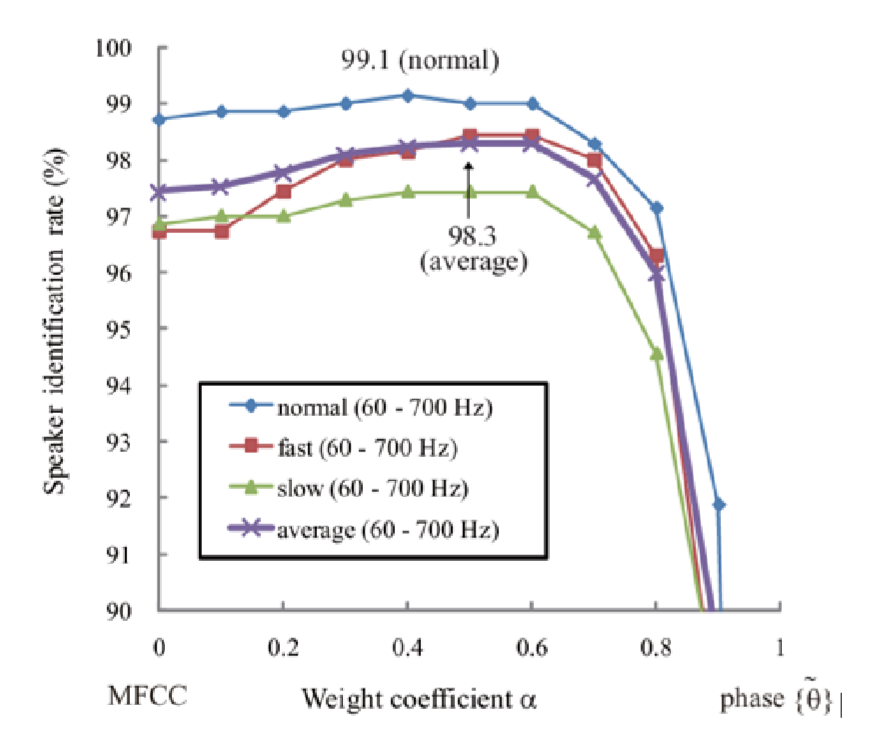
\includegraphics[width=4cm]{figures/1174095/tugas6/teori5.png}
            \centering
              \caption{Ilustrasi Membaca nilai Plot dari MFCC}
        \end{figure}
        
        \item One-hot Encoding
        \subitem one-hot encoding merupakan pemberian nilai pada suatu variabel jika nilai itu iya maka nilainya satu dan jika tidak maka nilainya nol.

        \begin{figure}[H]
            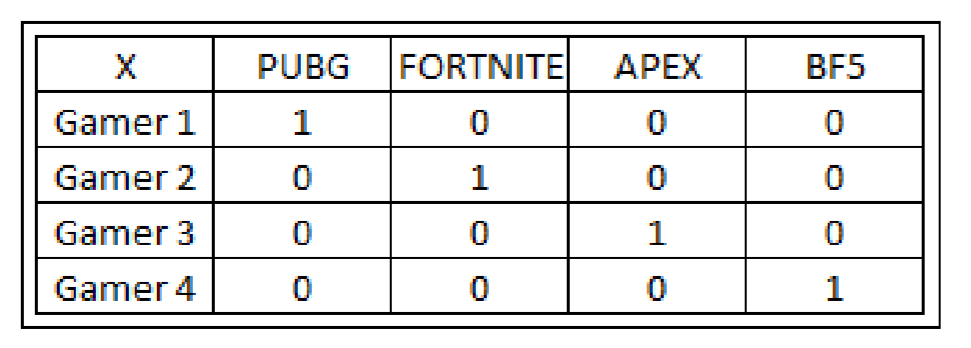
\includegraphics[width=4cm]{figures/1174095/tugas6/teori6.png}
            \centering
              \caption{Ilustrasi One-hot Encoding}
        \end{figure}
        
        \item fungsi dari np.unique dan to\_categorial dalam Code Program
        \subitem digunakan untuk membuat array sedangkan  to\_categorical digunakan untuk membuat matrix baui itu 64 bit atau 32 bit.
        
        \begin{figure}[H]
            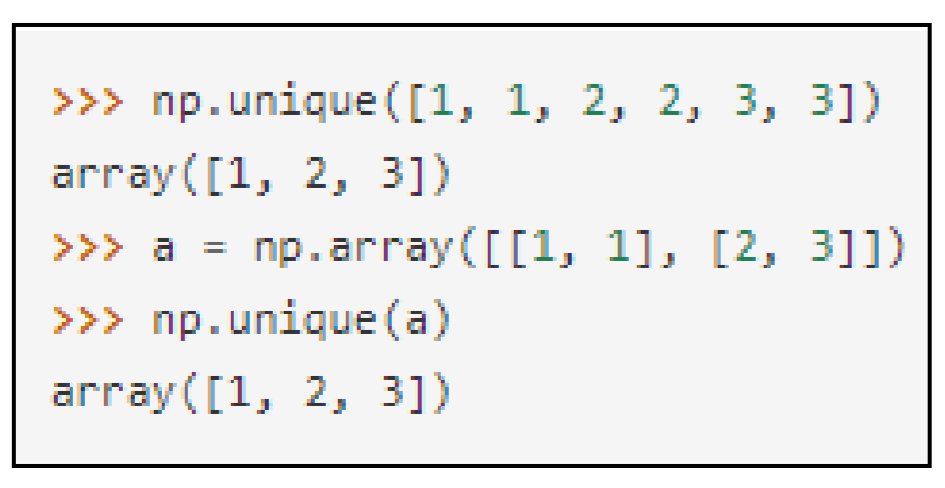
\includegraphics[width=4cm]{figures/1174095/tugas6/teori7.png}
            \centering
              \caption{Ilustrasi np.unique}
        \end{figure}
        
        \subitem sedangkan perintah to\_categorial adalah untuk membuat data integer yang terdeteksi untuk diubah menjadi data matrix biner. ilustrasi dapat dilihat pada gambar
        
        \begin{figure}[H]
            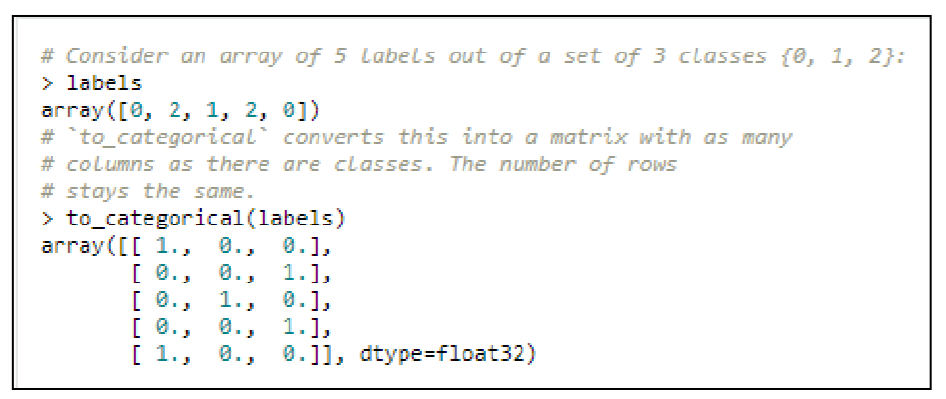
\includegraphics[width=4cm]{figures/1174095/tugas6/teori8.png}
            \centering
              \caption{Ilustrasi to\_categorial}
        \end{figure}
        
        \item fungsi dari Sequential
        \subitem sequential adalah prosesperbandingan setiap elemen satu persatu mulai dari dari objek pertama hingga yang di tuju atau jika mencari angka 100 maka sequential akan membagi bagian misalnya dari satu sampai 20 dan seterusnya sampai mendapat nilai seratus
        
        \begin{figure}[H]
            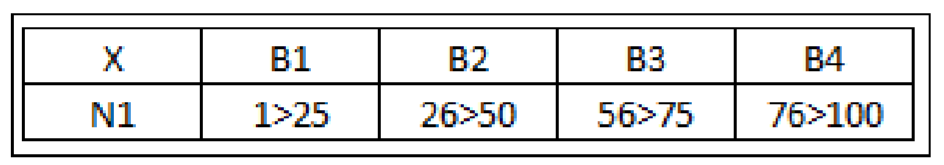
\includegraphics[width=4cm]{figures/1174095/tugas6/teori9.png}
            \centering
              \caption{Ilustrasi fungsi Sequential}
        \end{figure}
        \end{enumerate}

    \subsection{Praktek}
        \begin{enumerate}
            \item Penjelasan data GTZAN Genre Collection dan Freesound, Buat Code Program untuk Load data Tersebut.
            \subitem Isi data data merupakan datasets lagu atau suara yang tersiri dari 10 gendre yang di simpan kedalam 10 folder yaitu folder blues, classical, country, disco, hiphop, jazz, metal, pop, reggae, dan rock ke sepuluh folder tersebut masing-masing  berisi 100 data suara sedangkan data freesound merupakan contoh data suara yang akan di gunakan untuk menguji hasil pengolahan data tersebut dengan menggunakan metode mfcc. apakah suara dari freesound termasuk kategori jazz pop atau sebagainya.
            
            \subitem sedangkan Freesound merupakan sebuah contoh suara yang digunakan untuk menguji hasil dari pengolahannya dengan menggunakan metode MFCC, untuk mencari genre yang pas bagi contoh suara tersebut.
            
            \lstinputlisting[firstline=1, lastline=10]{src/1174095/tugas6/tugas6.py}
            
            \subitem Code tersebut digunakan untuk memanggil library Librosa yang memuat metode Feature dan Display yang akan digunakan untuk memproses data suara tersebut dengan MFCC. lalu Library Glob yang digunakan untuk mencocokan pattern yang spesifik dari data tersebut, Library Numpe yang digunakan untuk membuat data Vector, Library matplotlib yang digunakan untuk membuat data grafik dan Library Keras adalah open-source yang bekerja untuk memproses TensorFlow, CNTK dan Theano, yang didesain untuk melakukan penelitian dengan menggunakan Deep Neural Network.
            
            \item Penjelasan Code Program display\_mfcc
            
            \lstinputlisting[firstline=12, lastline=22]{src/1174095/tugas6/tugas6.py}
            
            \subitem dapat dilihat pada kode diatas pada baris kesatu dilakukan import librosa tang digunakan untuk fungsi mfcc pada suara. pada baris kedua dilakukan import librosa featuse dan pada baris ke tiga dilakukan librosa display selanjutnya pada baris ke empat dilakukan import glob kemudian insert numpy untuk pengolahan data menjadi vektor setelah itu dilakukan import matplotlib untuk melakukan ploting setelah itu dilakukan import librari keras
            
            \subitem dengan menggunakan code ini akan menampilkan hasil dari penggunaan display mfcc
            
            \lstinputlisting[firstline=24, lastline=25]{src/1174095/tugas6/tugas6.py}
            
            \subitem hasilnya adalah sebagai berikut, dengan menampilkan data dari file disco.00035.au dapat dilihat pada gambar
            
            \begin{figure}[H]
                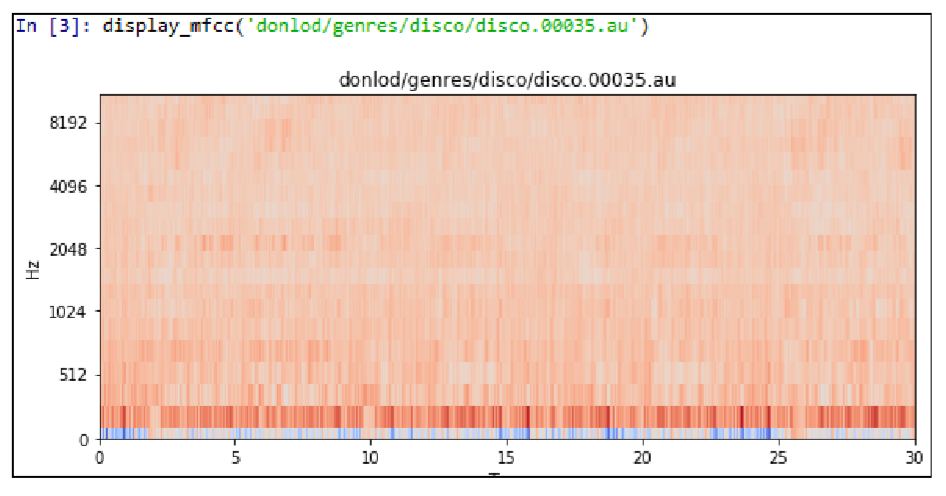
\includegraphics[width=4cm]{figures/1174095/tugas6/1.png}
                \centering
                  \caption{Hasil dari Code Program display\_mfcc}
            \end{figure}
            
            \item Penjelasan Code Program extract\_feature\_song
            
            \lstinputlisting[firstline=27, lastline=36]{src/1174095/tugas6/tugas6.py}
            
            \subitem pada baris ke tiga di definisikan nama extract\_features\_song yang nantinya akan di gunakan pada fungsi yang lainya kemudian dibuat variabel y dengan method librosa load setelah itu dibuat variabel baru mfcc dengan isi librosa features mfcc dengan isi variabel y tadi kemudian dibuat variabel mfcc dengan isian np.max dan variabel mfcc tadi terakhir di buat array dari data tersebut merupakan data 25000 data pertama. kenapa data 25000 pertama yang digunakan dikarenakan data tersebut digunakan sebagai data testing semakin besar data testing yang di gunakan maka semakin akurat hasil AI. tapi sebenarnya data tersebut relatif bisa lebih besar atau lebih kecil tergantung pada komputer masing masing.
            
            \begin{figure}[H]
                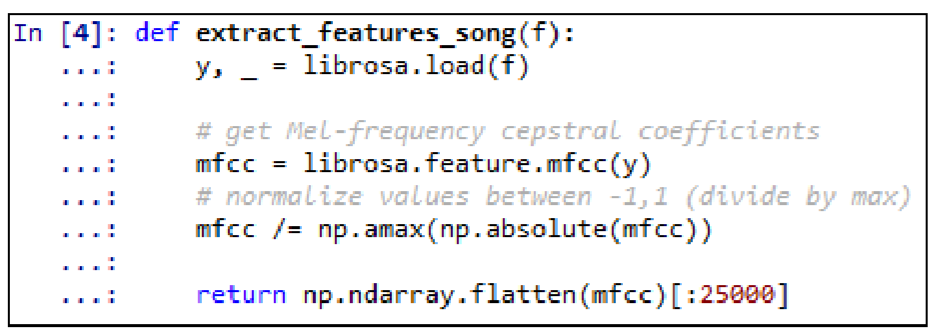
\includegraphics[width=4cm]{figures/1174095/tugas6/2.png}
                \centering
                  \caption{Code Program extract\_feature\_song}
            \end{figure}
            
            
            \item Penjelasan Code program  generate\_features\_and\_labels
            
            \lstinputlisting[firstline=38, lastline=56]{src/1174095/tugas6/tugas6.py}
            
            \subitem pada baris ke tiga merupakan pendefinisian nama fungsi yaitu generate features and labels kemudian membuat variabel baru dengan array kosing yaitu all\_features dan all\_labels kemudian mendefinisikan isian label untuk gendre dengan cara membuat variabel genres kemudian di isi dengan 10 gendre yang tadi setelah itu dilakukan fungsi if else dengan code for dan in setelah itu akan di buat encoding untuk data tiap tiap label contoh untuk blues 1000000000 dan untuk clasical 0100000000.
            
            \subitem hasil dari penggunaan perintah generate\_features\_and\_labels dapat dilihat pada gambar
            
            \begin{figure}[H]
                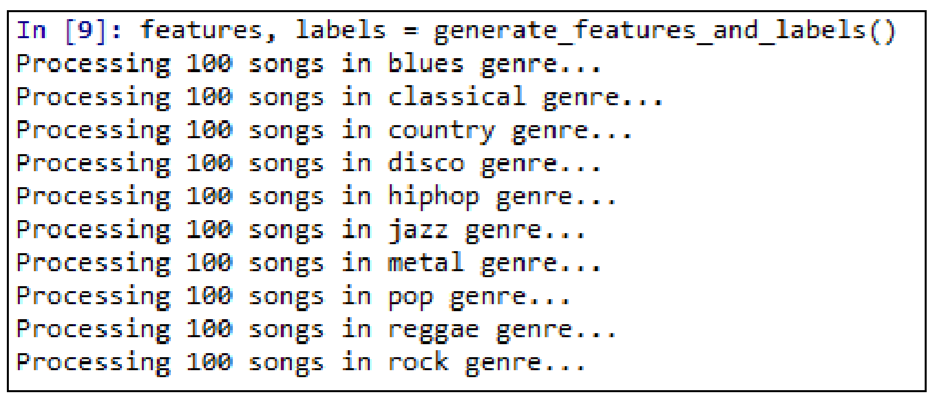
\includegraphics[width=4cm]{figures/1174095/tugas6/3.png}
                \centering
                  \caption{Code Program generate\_features\_and\_labels}
            \end{figure}
            
            \item Penjelasan tentang Kenapa proses pada generate\_features\_and\_labels lama
            
            \lstinputlisting[firstline=58, lastline=59]{src/1174095/tugas6/tugas6.py}
            
            \subitem halnini menjadi lama dikarenakan mesin membaca satupersatu file yang ada pada folder dan dalam foldertersebut terdapat 100 file sehingga wajar menjadi lama ditambah lagi mengolah data yang tadinya suara menjadi bentuk vektor. berikut merupakan codenya.
            
            \item Penjelasan tentang pembagian data training sebesar 80 persen.
            
            \lstinputlisting[firstline=65, lastline=66]{src/1174095/tugas6/tugas6.py}
            
            \subitem untuk code nya adalah sebagai berikut  yang merupakan code untuk membagi data sebanyak 80 persen untuk data training maka data musik tadi yang total jumlahnya 1000 akan di bagi dua untuk data training sebanyak 800  dan 200 untuk data testing.
            
            \begin{figure}[H]
                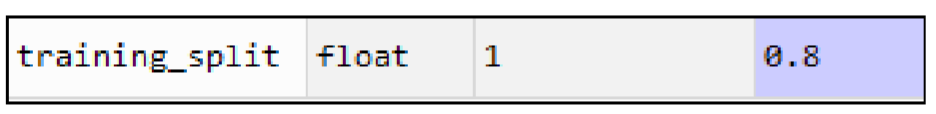
\includegraphics[width=4cm]{figures/1174095/tugas6/4.png}
                \centering
                  \caption{Hasil Code Program training\_split}
            \end{figure}
            
            \subitem dan berikut ini adalah hasil akhir dari data yang telah dipisahkan menjadi data TEST dan TRAIN dengan data tersebut sudah dilakukan SHUFFLE (acak) terdapat pada gambar.
            
            \begin{figure}[H]
                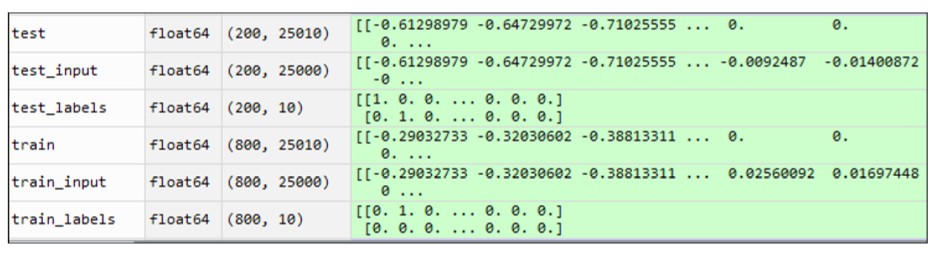
\includegraphics[width=4cm]{figures/1174095/tugas6/5.png}
                \centering
                  \caption{Hasil Code Program training\_split}
            \end{figure}
            
            \item Penjelasan parameter fungsi Sequential
            
            \lstinputlisting[firstline=92, lastline=98]{src/1174095/tugas6/tugas6.py}
            
            \subitem fungsi sequential digunakan untuk mengolah data inputan sesuai dengan fungsi yang ada pada fungsi sequential pada fungsi sequential kali ini menggunakan dua fungsi sequential mengkompile data dari 100 neuron atau dari 1 folder file dengan menggunakan fungsi relu dan softmax untuk menghasilkan outputan yang sesuai dengan keriteria.
            
            \subitem pada gambar dibawah ini adalah keluaran dari RUNNING code tersebut
            
            \begin{figure}[H]
                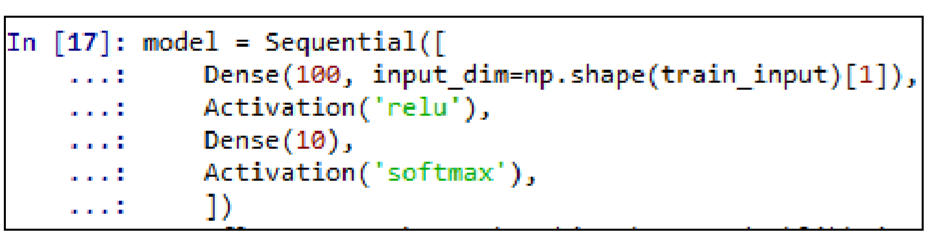
\includegraphics[width=4cm]{figures/1174095/tugas6/6.png}
                \centering
                  \caption{Hasil Code fungsi Sequential}
            \end{figure}
            
            \item Penjelasan parameter fungsi Compile
            
            \lstinputlisting[firstline=100, lastline=103]{src/1174095/tugas6/tugas6.py}
            
            \subitem fungsi kompile yang digunakan untuk mengetahui parameter yang digunakan dari data yang telah diolah untuk caranya dapat menggunakan codingan sebagai berikut.
            
            \begin{figure}[H]
                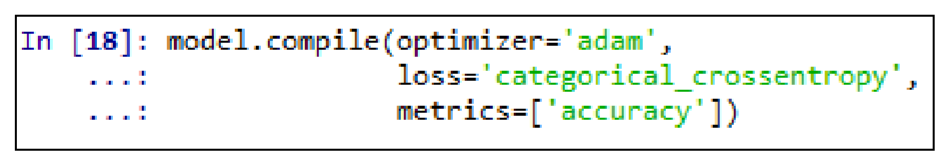
\includegraphics[width=4cm]{figures/1174095/tugas6/7.png}
                \centering
                  \caption{Hasil Code fungsi Compile}
            \end{figure}
            
            \subitem pada gambar dibawah ini adalah hasil dari penjelasan tentang data Sequential dan Compile
            
            \begin{figure}[H]
                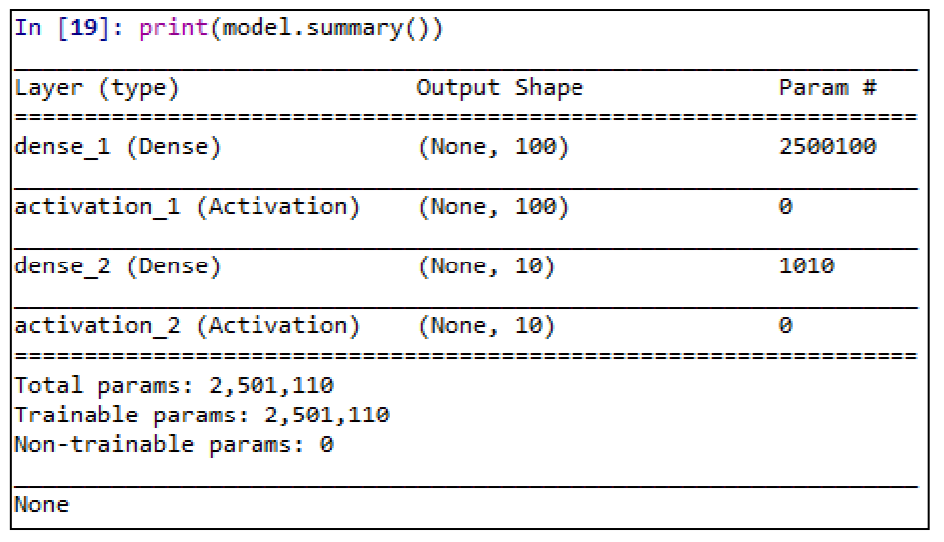
\includegraphics[width=4cm]{figures/1174095/tugas6/8.png}
                \centering
                  \caption{Hasil Code Program Summary}
            \end{figure}
            
            \item Penjelasan parameter fungsi Fit
            
            \lstinputlisting[firstline=107, lastline=109]{src/1174095/tugas6/tugas6.py}
            
            \subitem pada fungsi ini dilakukan pengolahan data dari 10 label tadi atau 10 file data sets tadi kemudian di hitung tingkat akurasi masing masing dan tingkat kegagalan atau loss data darisetiap file tersebut caranya dengan melakukan codingan berikut pada gambar tersebut menunjukan 10 pengolahan data untuk menentukan nilai akurasi dan loss dari data tersebut dan selanjutnya dilakukan fingsi evaluasi.
            
            \begin{figure}[H]
                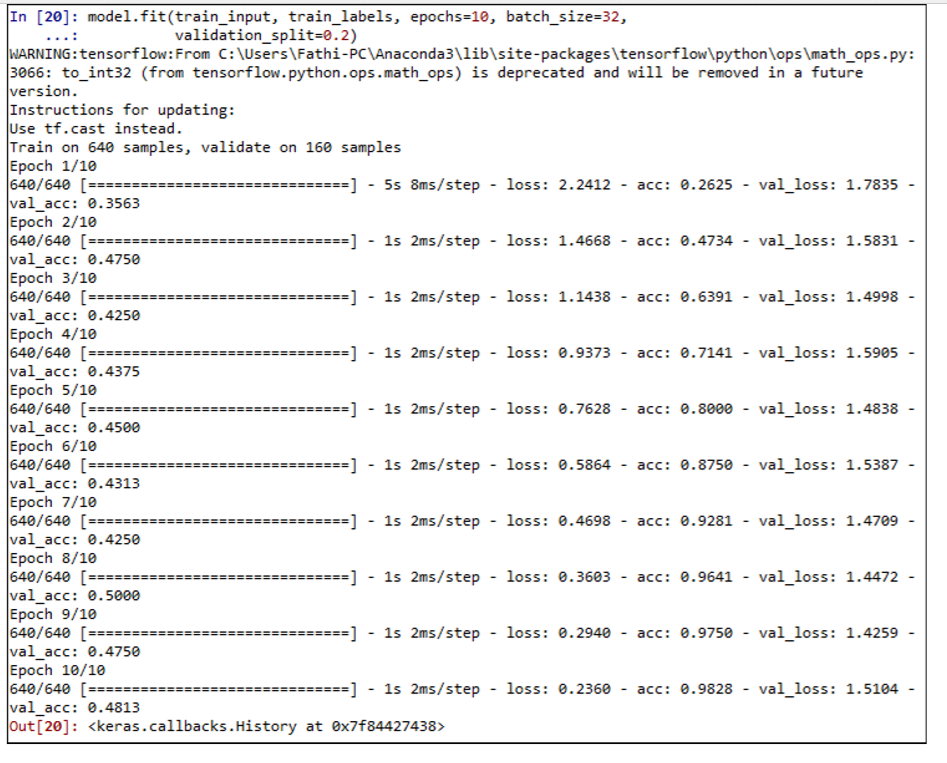
\includegraphics[width=4cm]{figures/1174095/tugas6/9.png}
                \centering
                  \caption{Hasil Code fungsi Fit}
            \end{figure}
            
            \item Penjelasan parameter fungsi Evaluate
            
            \lstinputlisting[firstline=111, lastline=112]{src/1174095/tugas6/tugas6.py}
            
            \subitem fungsi Evaluate digunakan untuk mengevaluasi data yang telah diolah dengan menggunakan perintah fungsi Seqeuntial, Compile dan juga Fit. untuk hasilnya dapat dilihat pada gambar.
            
            \begin{figure}[H]
                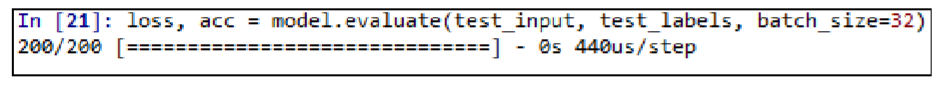
\includegraphics[width=4cm]{figures/1174095/tugas6/10.png}
                \centering
                  \caption{Hasil Code fungsi Evaluate}
            \end{figure}
            
            
            \lstinputlisting[firstline=114, lastline=116]{src/1174095/tugas6/tugas6.py}
            
            \subitem untuk data yang ditampilkan pada gambar dibawah ini adalah data yang telah disusun untuk membandingkan tingkat Akurasi dan Loss yang terjadi.
            
            \begin{figure}[H]
                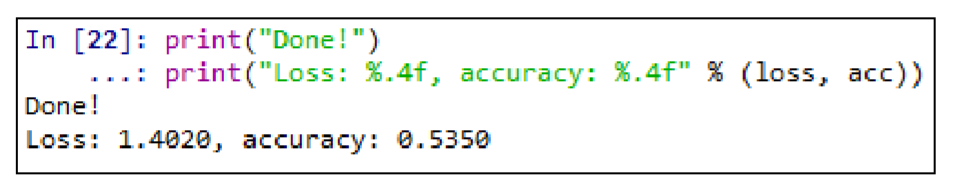
\includegraphics[width=4cm]{figures/1174095/tugas6/11.png}
                \centering
                  \caption{Hasil Code fungsi Evaluate}
            \end{figure}
            
            \item Penjelasan parameter fungsi Predict
            
            \lstinputlisting[firstline=118, lastline=119]{src/1174095/tugas6/tugas6.py}
            
            \subitem fungsi predic merupakan fungsi untuk membandingkan tingkat akurasi pada setiap label yang sepuluh tadi maka data akan di sandingkan ke masing masing tingkat akurasinya, yang akurasinya paling tinggi maka itulah jawaban untuk setiap inputan yang dilakukan. 
            
            \begin{figure}[H]
                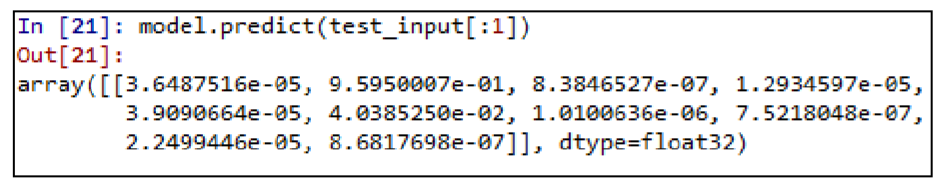
\includegraphics[width=4cm]{figures/1174095/tugas6/12.png}
                \centering
                  \caption{Hasil Code fungsi Predict}
            \end{figure}
            \end{enumerate}